\chapter{Big Data\label{ch:data}}

The LHC delivers $pp$ collisions at a very high rate, much higher than CMS can read out or store
offline. From all these collisions, CMS selects a subset of events many order of magnitudes smaller
which are the most relevant for the physics processes of interest. This task is accomplished
through the trigger system, which is discussed in Section~\ref{sec:trigger} both in general and
in the context of this analysis. The events selected by the trigger system compose the datasets
used by all CMS analyses. The worldwide computing grid for storage and processing of both datasets
and simulation samples is disussed in Section~\ref{sec:storage}. Finally, the simulation samples
employed by this analysis are discussed in Section~\ref{sec:sim}.


\section{The Trigger System\label{sec:trigger}}

The gap in time between successive bunch crossings by the LHC is 25 ns, which is equivalent to
a frequency of 40 MHz. This large rate is reduced by selecting only the most interesting events
in a two-level trigger system. The first level, Level 1 (L1), is hardward-based and reduceds the
total event rate from 40 MHz to 100 kHz~\cite{Bayatyan:706847}, whereas the second level,
the High Level Trigger (HLT) is software-based and reduces the total event rate from 100 kHz to
100 Hz~\cite{Virdee:1043242}. From here, the events are processed further and stored
for the physics analyses.

The L1 trigger attempts to identify basic physics objects based on coarse energy deposits in
ECAL or HCAL or
based on collections of hits in muon chambers. By scanning the energy deposited in the calorimeters,
quantities derived from the sum of energy deposited, such as the missing transverse energy $\met$.
The Level 1 global trigger (GT) combines these object candidates and derived quantities in order
to select events to pass the the HLT with a processing time of $3 \mu$s.
Up to 128 separate trigger paths may be supported.

The HLT is able to access more information than the L1 trigger, and in doing so it can provide
a better description of the event. At the HLT level, tracker information is used in conjunction with
the full granularity of ECAL and HCAL. Information at this level is based on the presence of one or
more candidate objects satisfying requirements based on their transverse momentum or energy and relative
or absolute positions in the detector. With this added complexity and fewer events to process,
the average processing time is 40 ms.

\subsection{The Trigger for $\ggbb$}

In the search for the $\ggbb$ final state, this analysis can be viewed as an extension of the
SM $\Hgg$ search~\cite{HggCMSpaper}. The excellent diphoton mass
resolution is the principle driver in the sensitivity since it allows for low background contamination
in the signal region, as will be shown in Chapter~\ref{ch:results}.
Therefore, the trigger strategy centers on the ability to find two high-quality photon candidates.

During 2012 data taking, the LHC luminosity increased over time, and the triggers at both L1 and HLT
had their thresholds increased in order to keep the event rates within the limits of the two levels.
The requirement at L1 is for two $e/\gamma$ candidates with $E_{\rm T}$ requirements of 13 (7) GeV
for the lead (sublead) candidate or for one $e/\gamma$ candidate with an $E_{\rm T}$ requirement of
22 GeV.

At HLT events are selected through diphoton triggers with asymmetric $E_{\rm T}$ thresholds
and complementary photon selections. One trigger selection requires a loose calorimetric
identification based on the shape of the electromagnetic shower and loose isolation requirements
on the photon candidates, while the other requires that the photon electromagnetic shower
is primarily concentrated in a three-by-three crystals super-cluster.
The trigger thresholds on the photon $E_{\rm T}$ are 26 (18) GeV and 36 (22) GeV on the leading
(subleading) photon, depending on the acquisition period of LHC data taking in 2012.
The path with the 26 (18) GeV thresholds is initiated by the L1 path with 13 (7) GeV thresholds, while
the path with 36 (22) GeV thresholds is initiated by the L1 path with a single 22 GeV threshold.

In addition to keeping the trigger rate within its limits, it is also neccessary to set thresholds
low enough such that the selection of signal events remains as high as possible. This trigger efficiency
is studied on Monte Carlo (MC) signal samples as well as on $Z\rightarrow e^+ e^-$ data.
For the study on MC, the efficiency is above 99.5\% for all conditions of 2012 data taking.

Figures~\ref{fig:ZeeTriggerPt} and \ref{fig:ZeeTriggerNvtx}
show how the trigger efficiency varies on data with respect to the
candidate photon $p_{\rm T}$ and the number of primary vertices in the event
using the tag and probe technique. To account for differences
between the shower shape between photons and electrons, the data sample was reweighted to match the
shower shapes. Within uncertainties, the trigger efficiency is higher than 99\% for the 2012 data.

\begin{figure}[ht]
 \begin{center}
    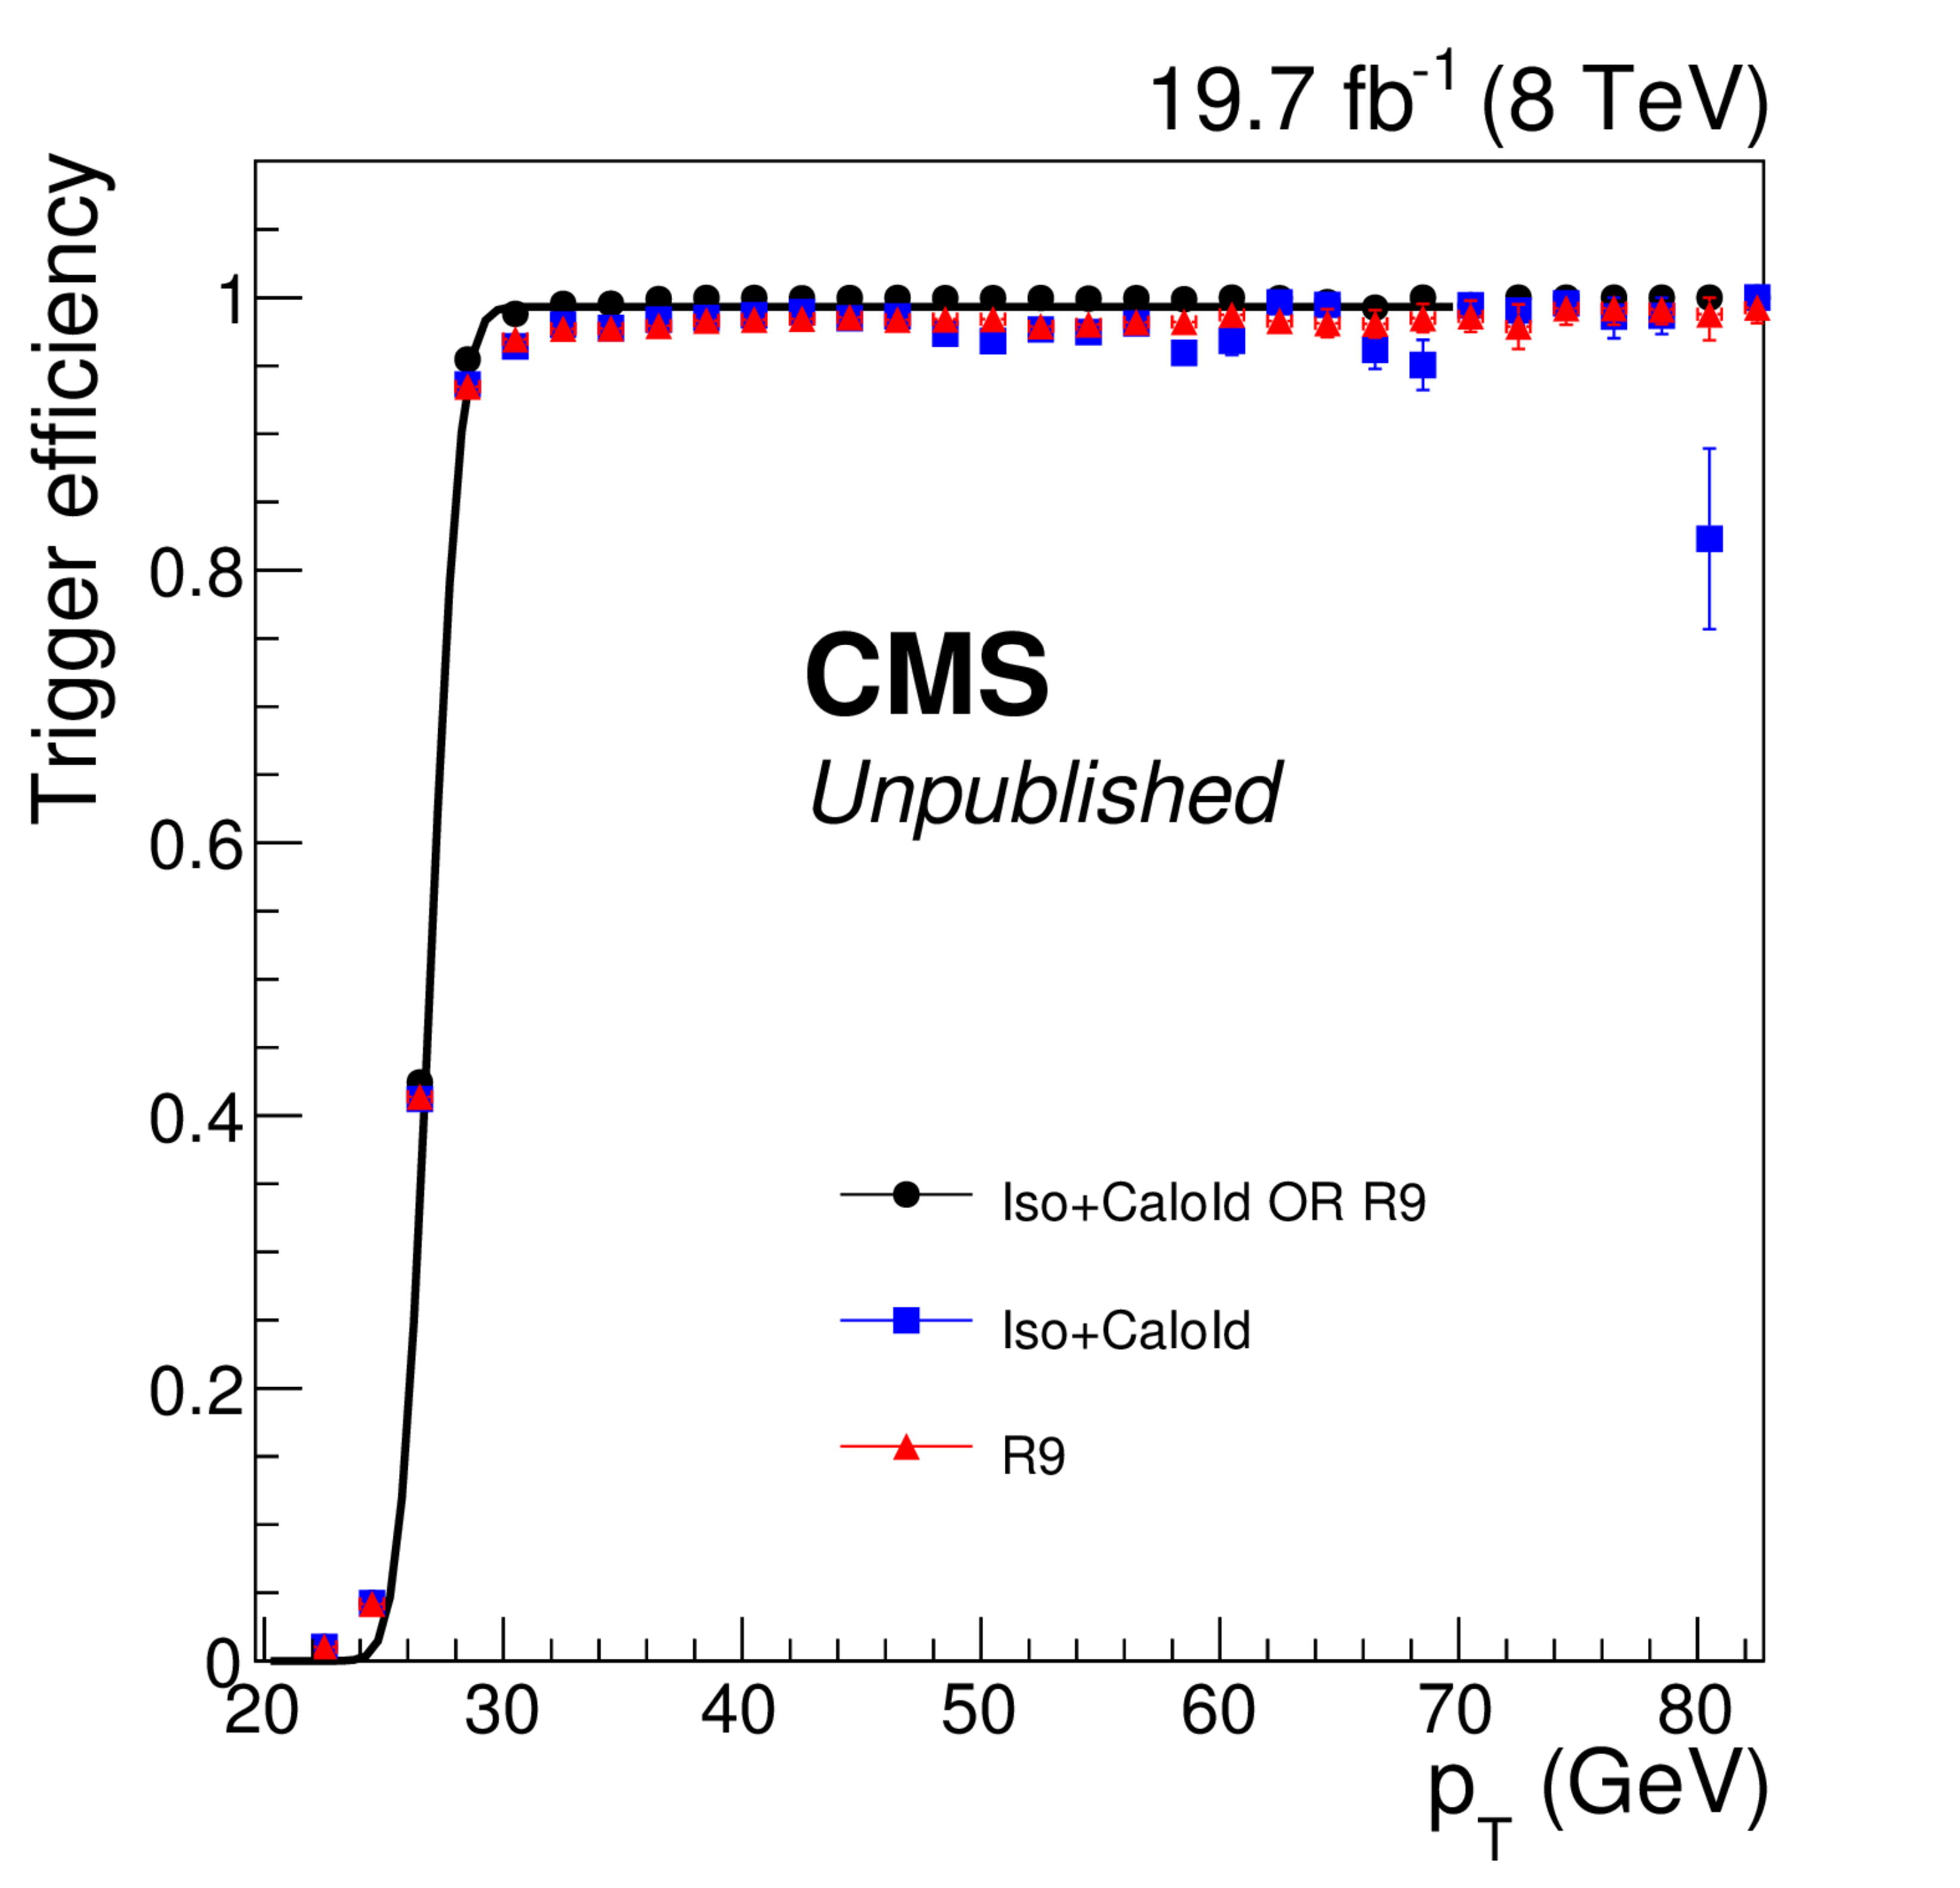
\includegraphics[width=0.60\textwidth]{figures/data/turnon_pt.pdf}
      \end{center}
\caption{Efficiency of the trigger selection as a function of the photon candidate transverse
momentum measured in $Z\rightarrow e^+ e^-$ events~\cite{HggCMSpaper}.}
\label{fig:ZeeTriggerPt}
\end{figure}

\begin{figure}[ht]
 \begin{center}
    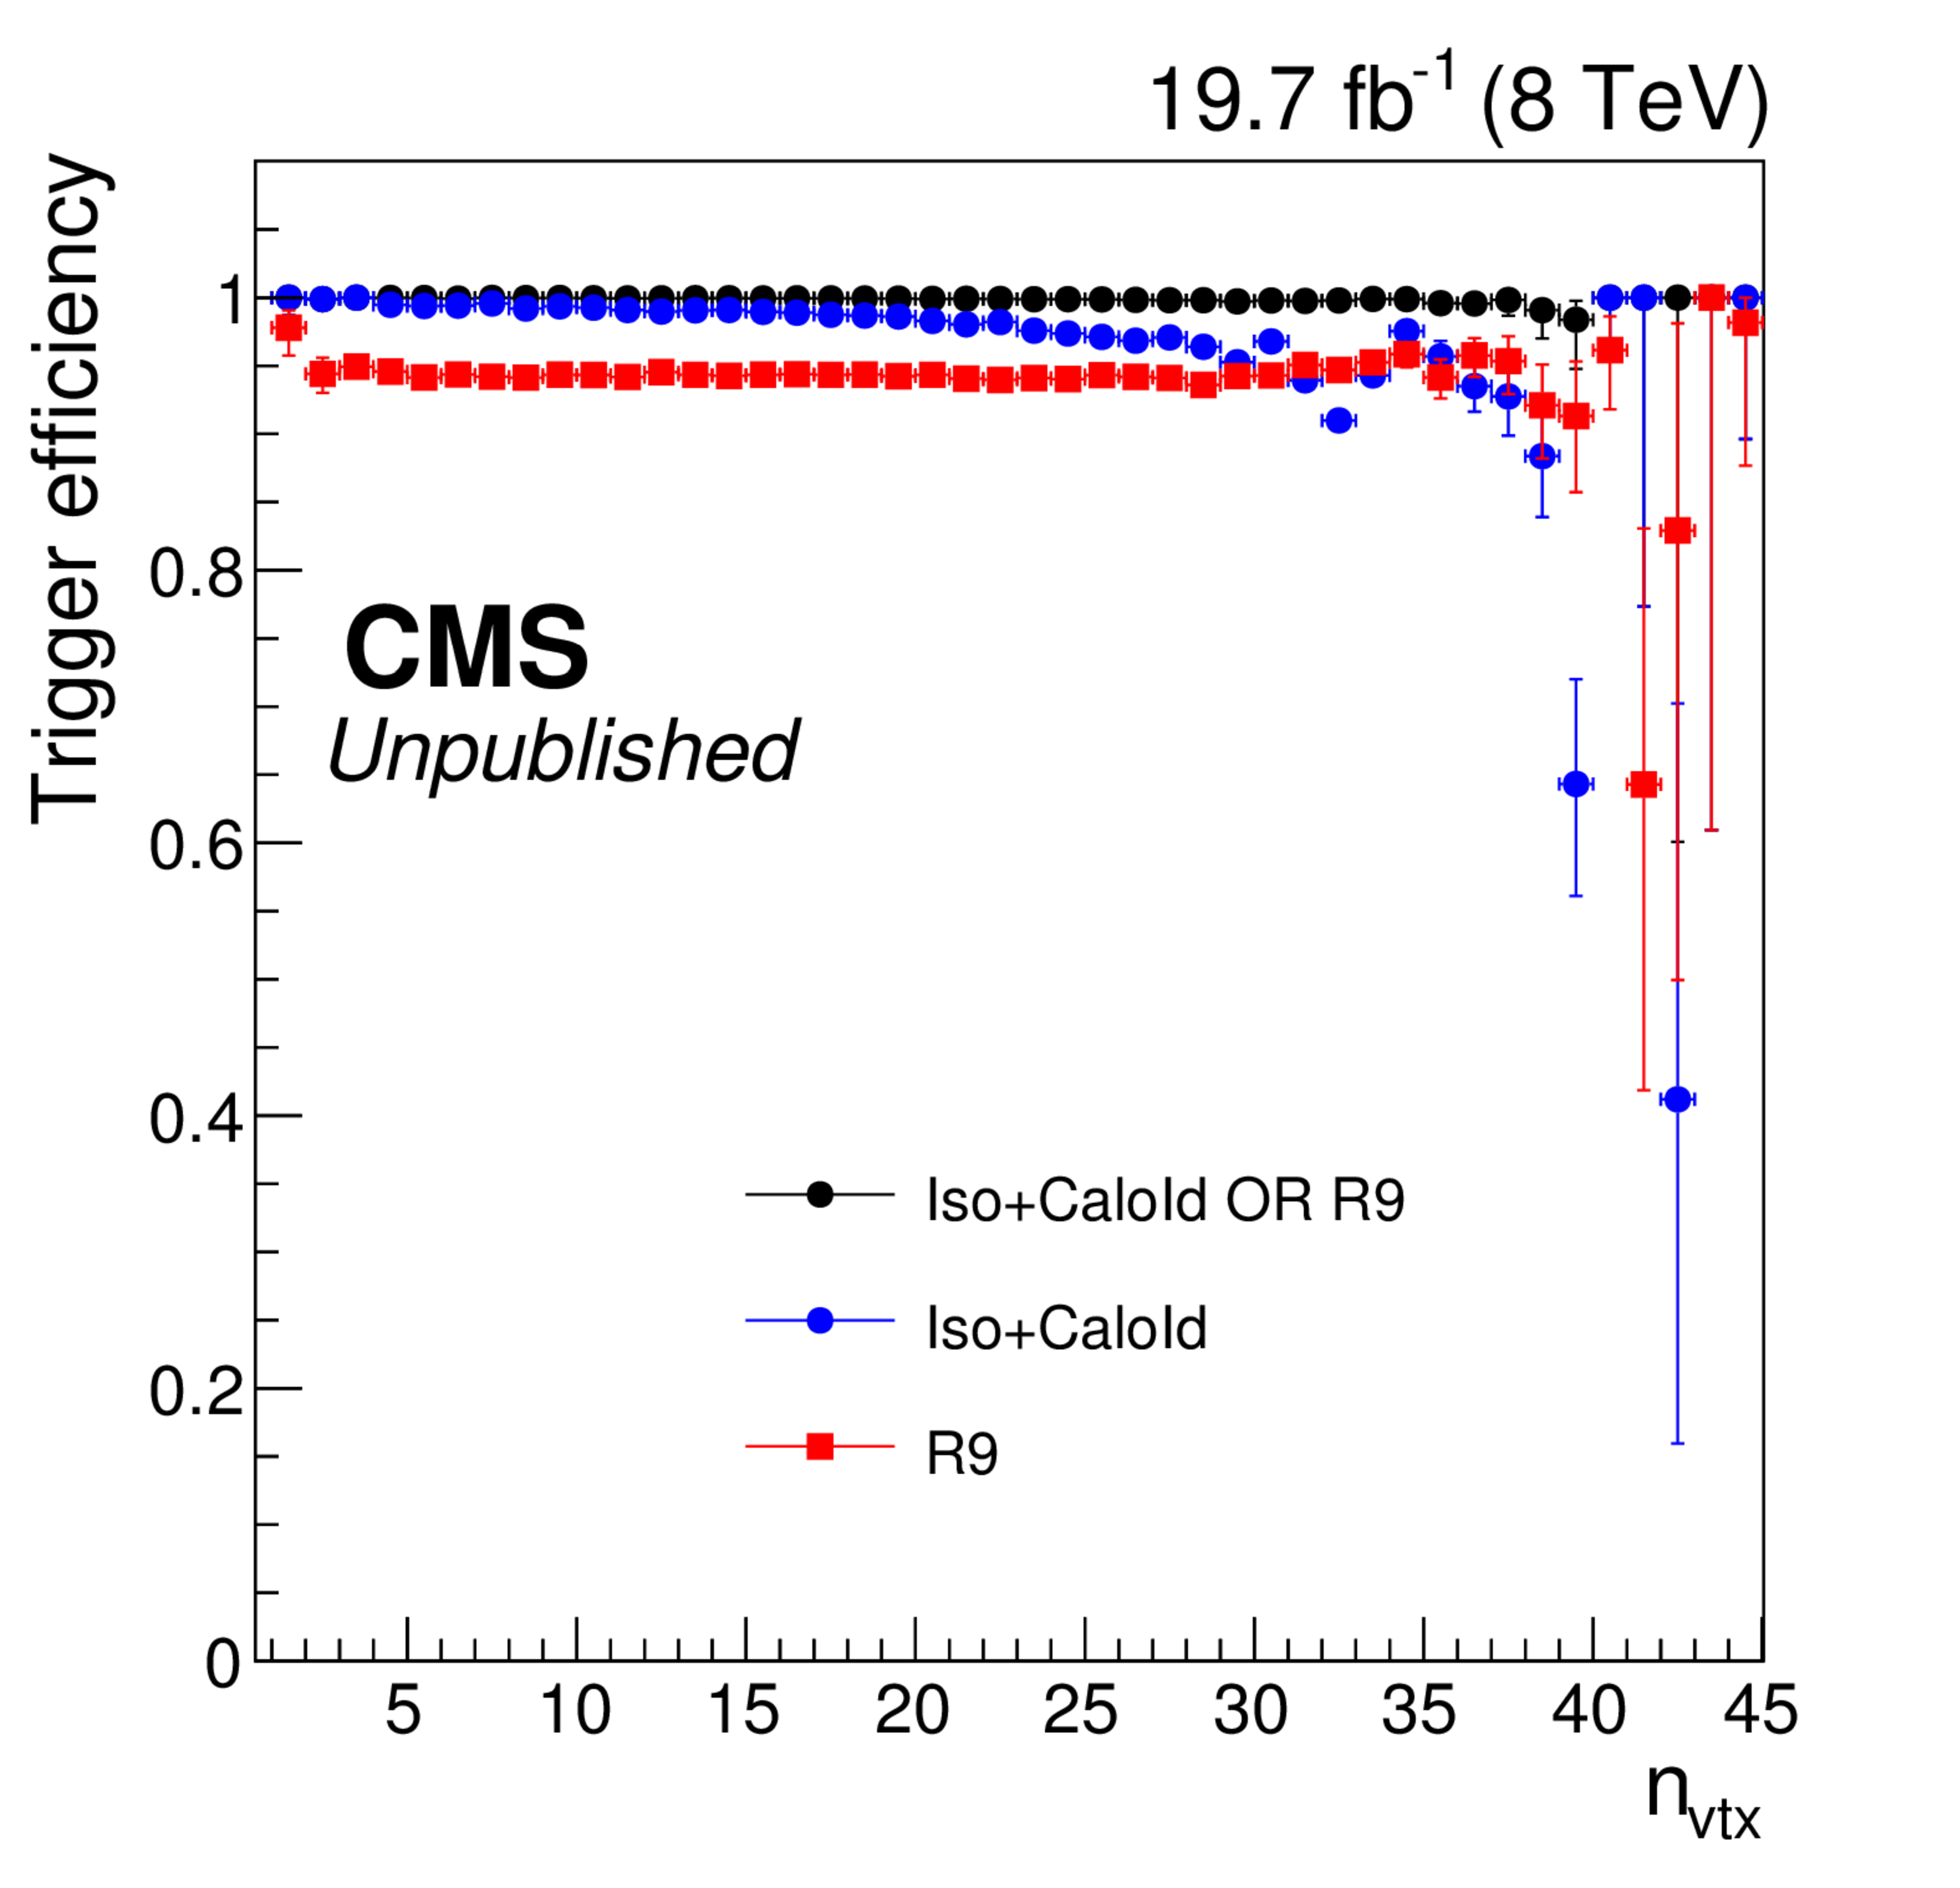
\includegraphics[width=0.60\textwidth]{figures/data/turnon_nvtx.pdf}
      \end{center}
\caption{Efficiency of the trigger selection as a function of the number of primary vertex in the event
measured in $Z\rightarrow e^+ e^-$ events~\cite{HggCMSpaper}.}
\label{fig:ZeeTriggerNvtx}
\end{figure}


\section{Data Storage Worldwide\label{sec:storage}}

All the data from the LHC and its experiments, including CMS, is processed, stored, and analyzed
in a distributed global collaboration of computing centers~\cite{Eck:840543}. The Worldwide
LHC Computing Grid (WLCG) is the world's largest computing grid, composing of over 170 centers
arranged in a tier structure. Part of this tier structure is shown in Figure~\ref{fig:cerncomputing}

\begin{figure}[ht]
 \begin{center}
    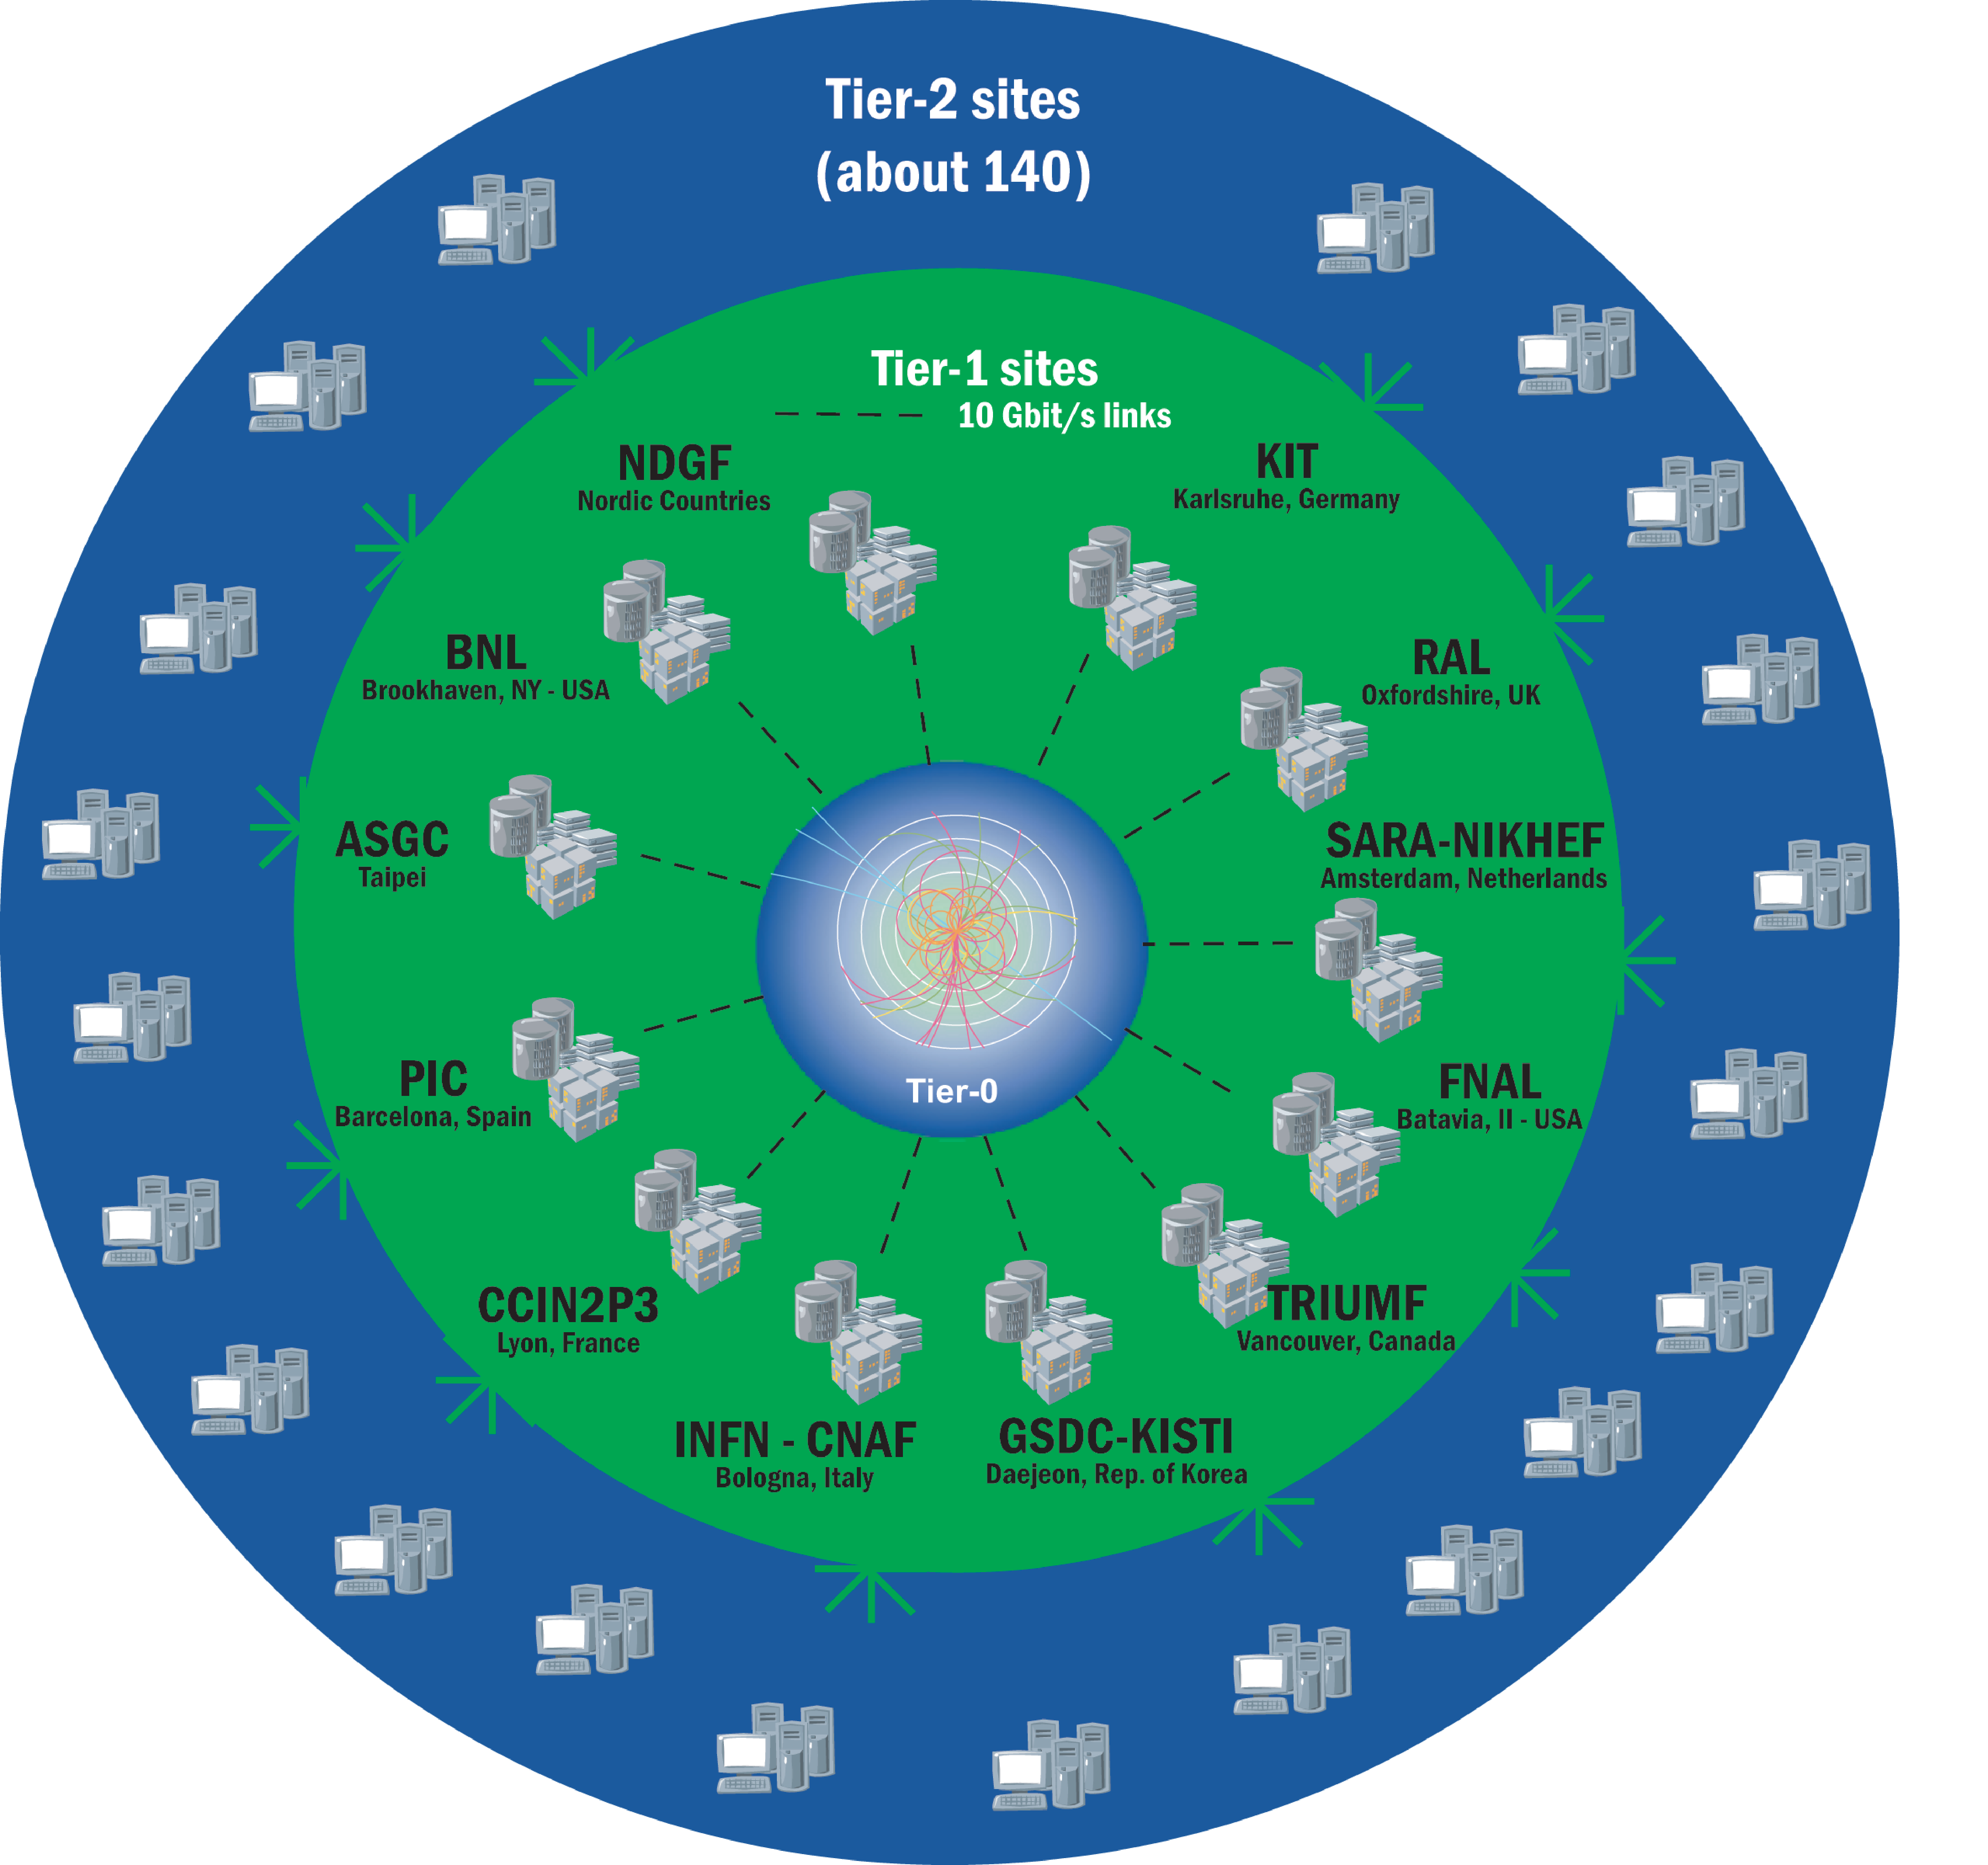
\includegraphics[width=0.70\textwidth]{figures/data/CCApr13-Tiers0-1-2_PNG-file.pdf}
      \end{center}
\caption{A schematic of the WLCG detailing the locations of the Tier-1 sites~\cite{cern:computing}.}
\label{fig:cerncomputing}
\end{figure}

Tier 0 is the CERN Data Center, through which all LHC data passes for initial processing and
reconstruction. The raw and processed data from Tier 0 is pushed to one of the 13 Tier 1 sites, where
later reprocessing and storage can be done. From here, the Tier 1 sites push the reconstructed
datasets to Tier 2 sites for storage and processing by analysts. This system handles the approximately
30 Petabytes of data generated per year by the LHC experiments in addition to the large amount of
MC samples generated and stored.

\section{Simulation Samples\label{sec:sim}}

%include more theory details on radion, graviton, mssm used in the sample generation

MC simulation samples are employed to study signal and background processes in more detail
than would be offered by data alone. In a search for some new signal process, there is a trade-off
between optimizing an analysis for one particular new physics scenerio and the ability to
generalize a result to other signal processes. This analysis generally searches for a double Higgs final
state by optimizing strategies separately between the resonant and nonresonant production mechanisms.
The signal MC samples are discussed in Subsection~\ref{subsec:sig_samples}.
In addition, good agreement between data
and background MC serves as a validation that the major backgrounds are understood and that
the data is behaving as expected. The background MC samples are discussed in
Subsection~\ref{subsec:bkg_samples}.

\subsection{Signal Simulation\label{subsec:sig_samples}}

\subsection{Background Simulation\label{subsec:bkg_samples}}


